\clearpage
\blankpage
\vspace*{\fill}
\begin{figure}[H]
    \centering
      
\includegraphics[width=5cm]{src/cover/title_page_colorspace.png}%
\end{figure}
\vspace*{\fill}
\thispagestyle{empty}%
\clearpage
\blankpage

\chapter{developing a bit of a complex}
\begin{definition}[Jeffrey Says]
\setlength{\intextsep}{0pt}%
\setlength{\columnsep}{3pt}%
\begin{wrapfigure}{l}{0.12\textwidth}

\includegraphics[width=\linewidth]{src/callout/psych.png} 
\end{wrapfigure}
\small
This was the next major evolution of the lightsynth. The Atari machine had a
  much more extensive palette than the Commodore machines, plus you could make
  all kinds of interesting screen modes using the Display List Interrupt
  system, so it seemed like a natural machine to develop a next-generation
  lightsynth on. I still used the same basic algorithm as Psychedelia, but
  introduced a lot more colour variation, and colour cycling. There was also a
  provision for designing static graphics and logos on the screen and having
  the generated patterns flow over or under them, and many more symmetry modes
  afforded by the flexible hardware. Screens could have a cylindrical "curved"
  look since you could vary the vertical pixel size on a scanline by scanline
  basis, thanks to the DLIs.
\end{definition}
Just a few months before the mini-version of \textit{Psychedelia} included in \textit{Batalyx} appeared, Minter released
his next major iteration in his life-long sequence of light synthesizers. This was \textit{Colourspace} and it was a major
improvement on its predecessor. The core code of the game remained  the
same (the algorithms we have covered in detail in Psychedelia remain unchanged) but the hardware of the
Atari 8 bit computers created opportunities for much more colour and complexity.

For this reason alone it is worth us devoting the final parts of this book to the effects of this second generation
in the series. There will be much less code for us to cover because so much of it was simply dropped in from 
\textit{Psychedelia}. The important, and interesting, differences lie mainly in the work required to take advantage of the
Atari 400/800's graphical capabilites. These we will cover in our next chapter 
\hyperref[sec:painting]{\textcolor{blue}{'painting pixels is so complicated'.}} 
There we'll take a look at some of the things Minter had to learn about the Atari and adapt
to the purpose of making a new generation of Psychedelia and this will give us a clear sense of 
the scale of the undertaking in such a short time.

\clearpage
\begin{figure}[H]
    \centering
    \begin{adjustbox}{width=12cm,center}
    \frame{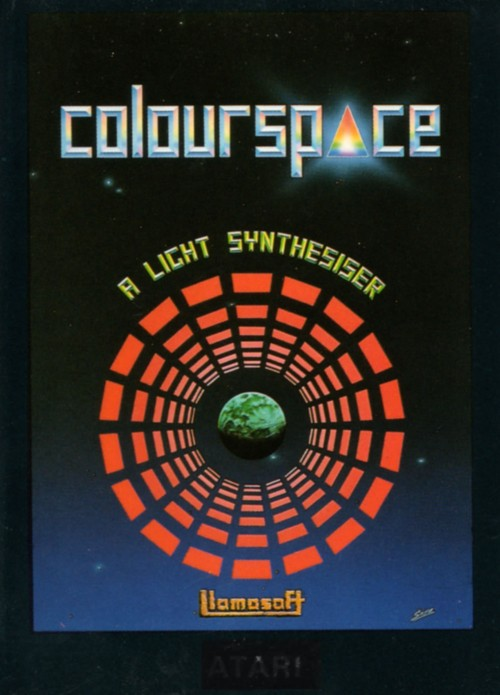
\includegraphics{src/preface_colorspace/colorspace.jpg}}%
    \end{adjustbox}
\caption{Cover art by Steinar Lund for the commercial edition of Colourspace}
\end{figure}
\clearpage
After that we are free to appreciate the fruit of this Atari port without detaining ourselves too long over the code
required to achieve it since we have already seen it in action in our previous chapters on \textit{Psychedelia}.
For this reason our final chapters provide a restful close to this book in which we can enjoy the colours
and configurations of \icode{Colourspace} and I can get away with as little writing as possible.
\hyperref[sec:lightforms]{\textcolor{blue}{'all the little lightforms'}}
sets out the 28 new patterns available
in \textit{Colourspace}, while 
\hyperref[sec:colourspace_presets]{\textcolor{blue}{'plentiful presets'}}
shows off all 78 presets. Finally, in
\hyperref[sec:colourflow]{\textcolor{blue}{'colourflow'}} we get to see the full range of colour schemes
the game employs.

  



